\paragraph{Z-test}
It says how many SEs away an observed value is from its expected value,
where the expected value is calculated using the null hypothesis.
\begin{center}
	$z=\dfrac{\text{observed}-\text{expected}}{\text{SE}}$
\end{center}
\paragraph{T-test}
\begin{center}
	$t=\dfrac{\text{average of draws}-\text{c}}{\text{SE}}$
\end{center}
$c$ corresponding to the constant which is fixed in $H_{0}$\\
As the number degrees of freedom increases the curves get closer and 
closer to the normal.
\paragraph{Test Method}
\begin{figure}[H]
	\begin{center}
		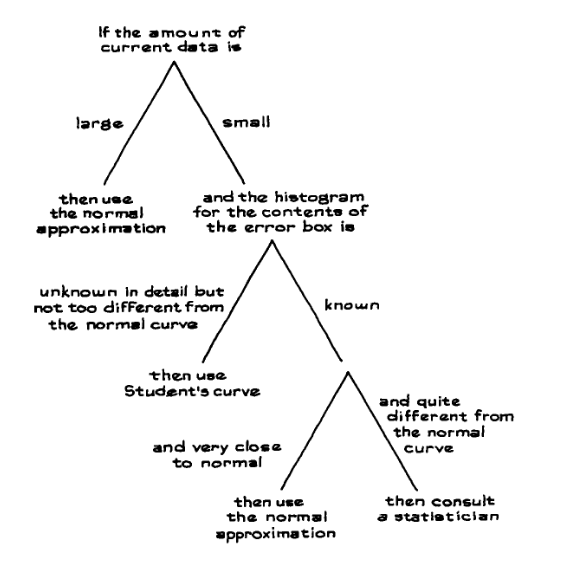
\includegraphics[width=.5\textwidth]{./chaps/27sec/images/1_methodApproxNorm.png}
	\end{center}
	\caption{Procedure when testing}
	\label{fig:1_mehtodeApproxNorm}
\end{figure}
